%!TEX TS-program = xelatex
\documentclass[]{friggeri-cv}
\usepackage{graphicx,txfonts}
\newcommand{\heart}{\ensuremath\varheartsuit}
\DeclareSymbolFont{extraup}{U}{zavm}{m}{n}
\DeclareMathSymbol{\varheart}{\mathalpha}{extraup}{86}
\DeclareMathSymbol{\vardiamond}{\mathalpha}{extraup}{87}

\begin{document}
\header{Pawe\l{}}{Kordowski}
       {junior python developer}

\begin{abstract_pk}
I am a Python developer with one year of experience. Because of my physics backgorund I like math theories especially grpah theory and data mining. Personally I am a sport oriented outgoing guy and team player.
\end{abstract_pk}

% In the aside, each new line forces a line break
\begin{aside}
  \section{contact}
    +48 503 302 537
    \href{mailto:paw.mar.kor@gmail.com}{paw.mar.kor@gmail.com}
    \href{http://stackoverflow.com/users/2999347/pmkor}{stackoverflow://pmkor}
    \href{http://facebook.com/pmkor}{fb://pmkor}
  \section{languages}
    polish native
    english C1
    german B2
    lesser polish dialect A2
  \section{programming}
    {\color{red} $\heart$} Python {\color{red} $\heart$}
    MATLAB
    basic JavaScript \& Scala
    in the past Java \& C++
  \section{python libs}
   mako, CherryPy
   SQLAlchemy engine
   OpenERP, numpy
   matplotlib, wxPython
   Celery basics
   Pyramid basics
   Flask basics
   \section{databases}
    PostgreSQL, SQLite
  \section{linux}
    intermediate bash scripting
   basic awk, xargs
  flock, grep, ps, etc.
  \section{technologies}
   REST API, GraphQL DataLoader
    git(hub/lab/flow), jira, confluence
    jenkins, rundeck, Ansible
   Amazon Web Service
   (EC2, RDS, Cloudwatch cli, boto3)
   logstash, PyCharm DataGrip
   \LaTeX
\end{aside}

\section{experience}

\begin{entrylist}
%\subsection{Full Time}\\
  \entry
    {06.2017 - Now}
    {\href{http://daftcode.pl/}{Daftcode sp. z o.o.}}
    {Warsaw, Poland}
    {\textit{Junior Python Developer}\\
    I'm a member of a team working on a payment backend application. Most of my tasks are app's logging stack (Sentry, Fluent) maintenance and refactoring small parts of the Pyramid application. While working in Daftcode I learned basics of Pyramid and Celery.}
  \entry
    {04.2017 - 06.2017}
    {\href{https://evojam.com/}{Evojam sp. z o.o.}}
    {Warsaw, Poland}
    {\textit{Junior Python Developer}\\
    I was a backend python developer working on the outsourced project matching companies looking for services with service providers. I was responsible for maintaining, bugfixnig and developing REST based microservices. While working in Evojam I learned GraphQL, DataLoader, JS and Node.js basics. My main activity was supporting the frontend team. I had an opportunity to play with NoSQL databases (redis, elasticsearch). The main task I finished was migrating the project from REST to GraphQL.}
  \entry
    {06.2015 - 04.2017}
    {\href{http://www.syncron.com/}{Syncron Poland sp. z o.o.}}
    {Warsaw, Poland}
    {\textit{Application Specialist}\\
    As a member of Software Automation team I was developing tools for internal use. My work was focused on Syncron's products monitoring, automation of AWS servers management and data application input integration using ETL tool Talend. I've created a CherryPy based web application for log analysis and crawlers frequently inserting database statistics and daily summaries into Confluence. While working in Syncron I learned Ansible and I realized that taking care of small things is very important.}
  \entry
    {10.2014 - 06.2015}
    {\href{http://www.lacan.com.pl/}{Lacan Technologies sp. z o.o.}}
    {Warsaw, Poland}
    {\textit{Junior Python Developer}\\
    I was working on ERP/CRM application modules using OpenERP framework.}
  \entry
    {10.2012 - 10.2014}
    {\href{http://www.lin-magdeburg.de/}{Leibniz Institute for Neurobiology\\Non-Invasive Brain Imaging Special Lab}}
    {Magdeburg, Germany}
    {\textit{PhD internship}\\
    I was developing a new algorithm for brain signal analysis solving source localization problems using MATLAB and Python for data analysis and visualization.}
%\subsection{Part Time}\\
  \entry
    {09.2011 - 06.2012}
    {\href{http://wlh.edu.pl/}{Wielokulturowe Liceum Humanistyczne im. Jacka Kuronia}}
    {Warsaw, Poland}
    {\textit{math teacher}\\
    All my students passed the math matura exam despite the fact it was the very first time it was compulsory and students were art and literature oriented.}
\end{entrylist}

\newpage

\section{opensource contribution}

\begin{entrylist}
  \entry
    {2016}
    {\href{https://weather.fundin.pl/}{weather.fundin.pl}}
    {\href{https://bitbucket.org/jt1/weather_history}{bitbucket repo}}
    {Small Django web application for aggregating weather data written in order to help assess avalanche and winter climbing risk. This is my friend's idea, I'm the second contributor.}
\end{entrylist}

\section{education}

\begin{entrylist}
  \entry
    {2011 – 2016}
    {Doctor {\normalfont of Philosophy in Medical Physics}}
    {University of Warsaw, Faculty of Physics}
    {\textit{Multivariate matching pursuit analysis of MEG evoked fields}\\
    In the thesis I developed a new method for localization of brain activity.}
  \entry
    {2006 – 2011}
    {Master {\normalfont of Science in Medical Physics}}
    {University of Warsaw, Faculty of Physics}
    {\textit{Event related synchronization and desynchronization of MEG signal in linguistic experiment}\\
    In the thesis I investigated brain activity during linguistic experiment using well known algorithms.}
\end{entrylist}

\section{conferences}

\begin{entrylist}
  \entry
    {2014}
    {Poster}
    {19th International Conference on Biomagnetism (BIOMAG 2014), Halifax, Canada}
    {Spatio--temporal dictionaries for Multivariate Matching Pursuit decomposition of evoked brain responses in MEG}
  \entry
    {2014}
    {Oral Presentation}
    {Neuronus 2014 IBRO \& IRUN Neuroscience Forum, Cracow, Poland}
    {Spatio--temporal dictionaries for Multivariate Matching Pursuit decomposition of evoked brain responses in MEG}
  \entry
    {2012}
    {Poster}
    {8th FENS Forum of Neuroscience, Barcelona, Spain}
    {Event related desynchronization and synchronization in linguistic experiment}
\end{entrylist}

\section{publications}
\subsection{articles in peer-reviewed journals}
\begin{entrylist}
  \entry
    {2017}
    {Simultaneous spatio-temporal matching pursuit decomposition of evoked brain responses in MEG.}
    {Biological cybernetics}
    {Kordowski P., Matysiak A., K\"onig R. and Sielu\.zycki C.}
  \entry
    {2014}
    {Implementation of a dose gradient method into optimization of dose distribution in prostate cancer 3D-CRT plans.}
    {Reports on practical oncology and radiotherapy}
    {Gi\.zy\'nska M., Kuko\l{}owicz P. and Kordowski P.}
  \entry
    {2014}
    {Maximum-likelihood estimation of channel-dependent trial-to-trial variability of auditory evoked brain responses in MEG.}
    {Biomedical engineering online}
    {Sielu\.zycki C. and Kordowski P.}  
    \entry
    {2012}
    {Estimation of the spatiotemporal structure of event-related desynchronization and synchronization in magnetoencephalography.}
    {Journal of neuroscience methods}
    {\.Zygierewicz J., Sielu\.zycki C., Zacharias N., Suffczy\'nski P., Kordowski P., Scheich H., Durka, P. and K\"onig, R.}
\end{entrylist}

\newpage

\section{interests}
{\textbf{professional:} data analysis, graph theory, functional programming \textbf{personal:} caving, climbing, spending time with my dog, enduro biking, mountain running, slacklining, brain teasers, meeting new people, dreaming}

\begin{center}
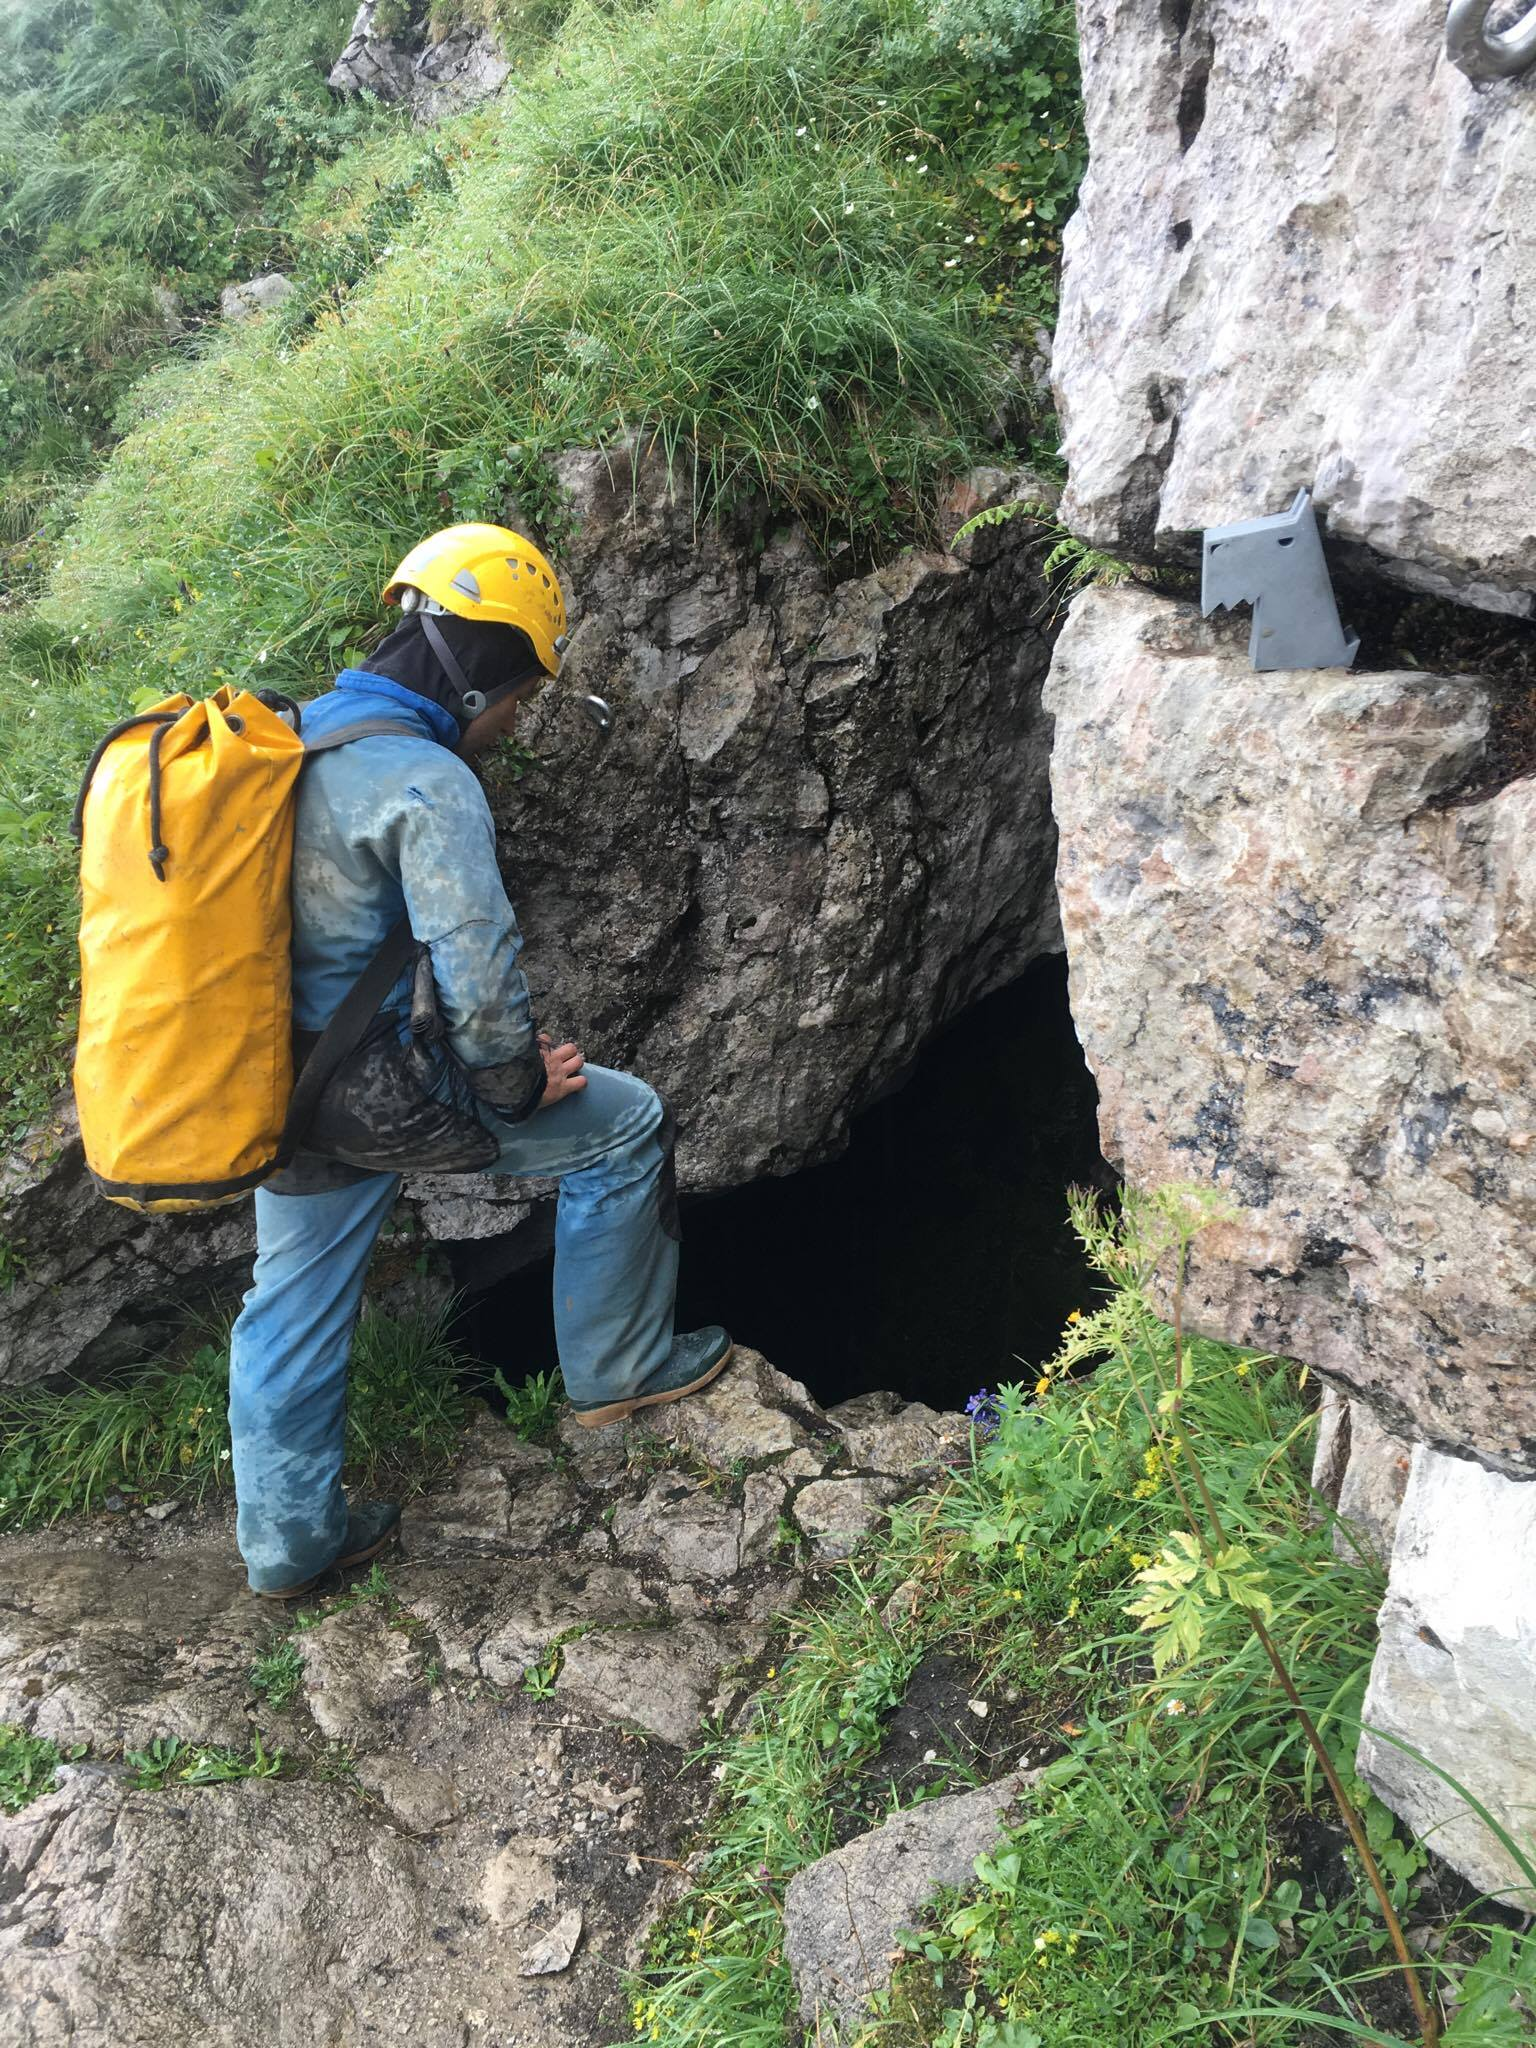
\includegraphics[width=0.3\textwidth]{foto1}
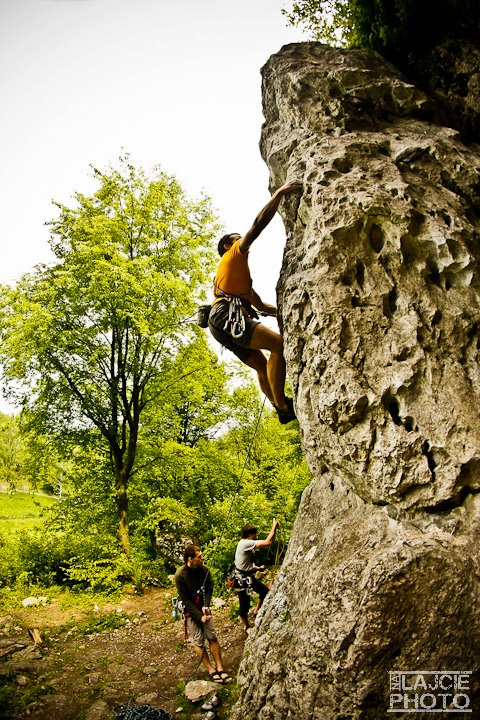
\includegraphics[width=0.3\textwidth]{foto4}
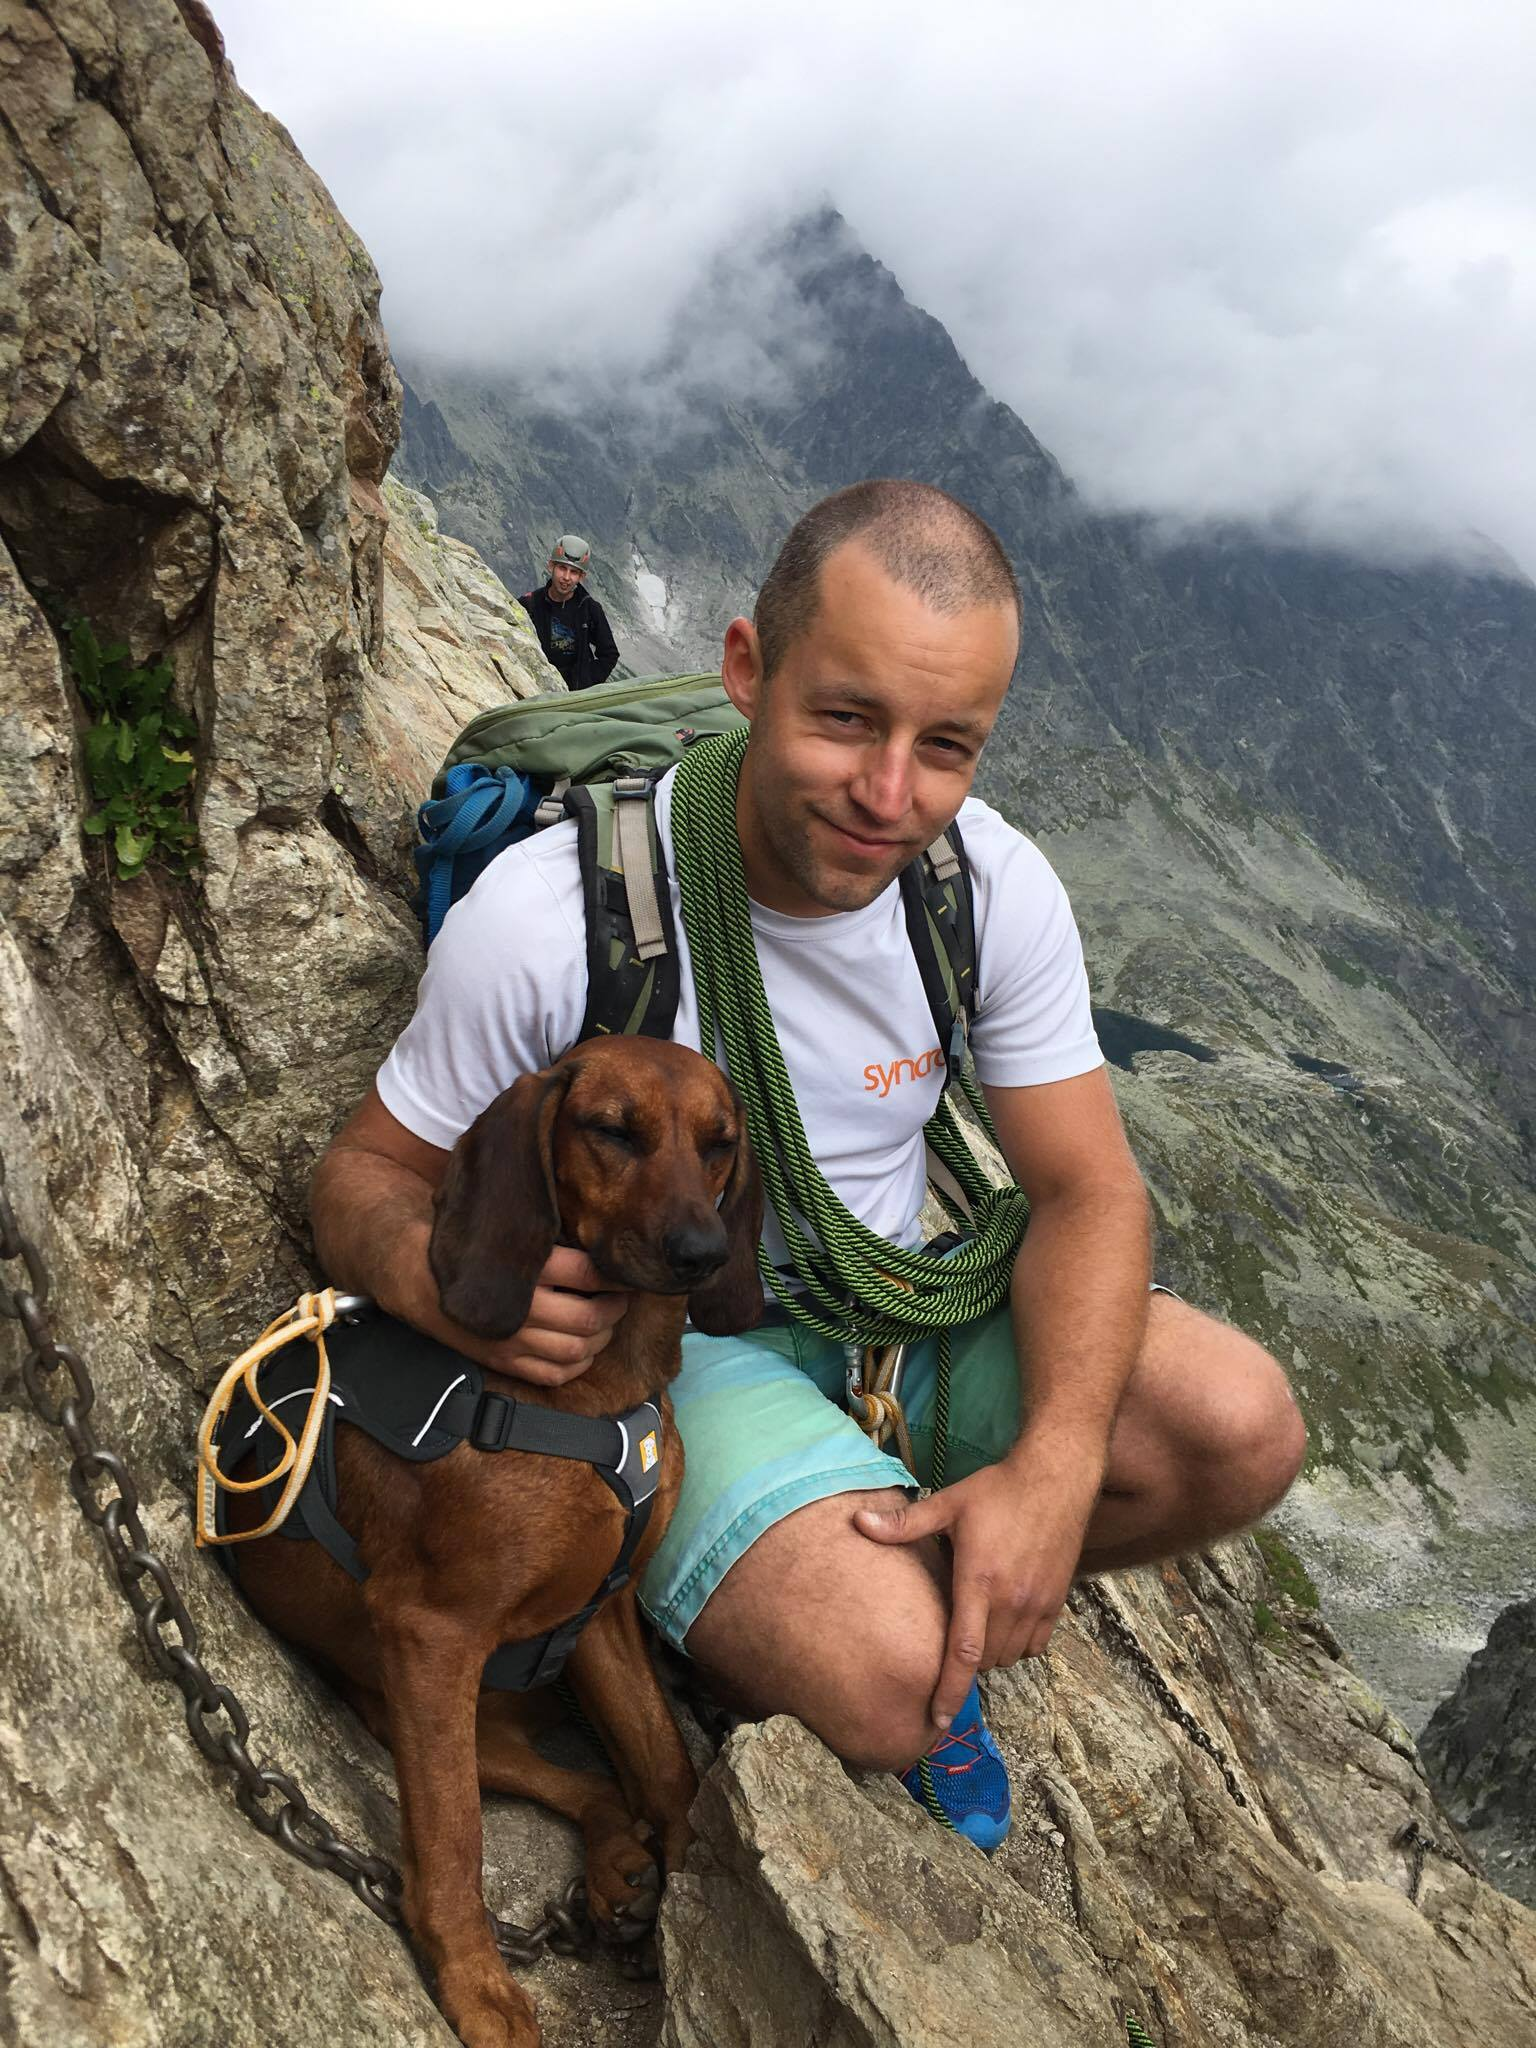
\includegraphics[width=0.3\textwidth]{foto}
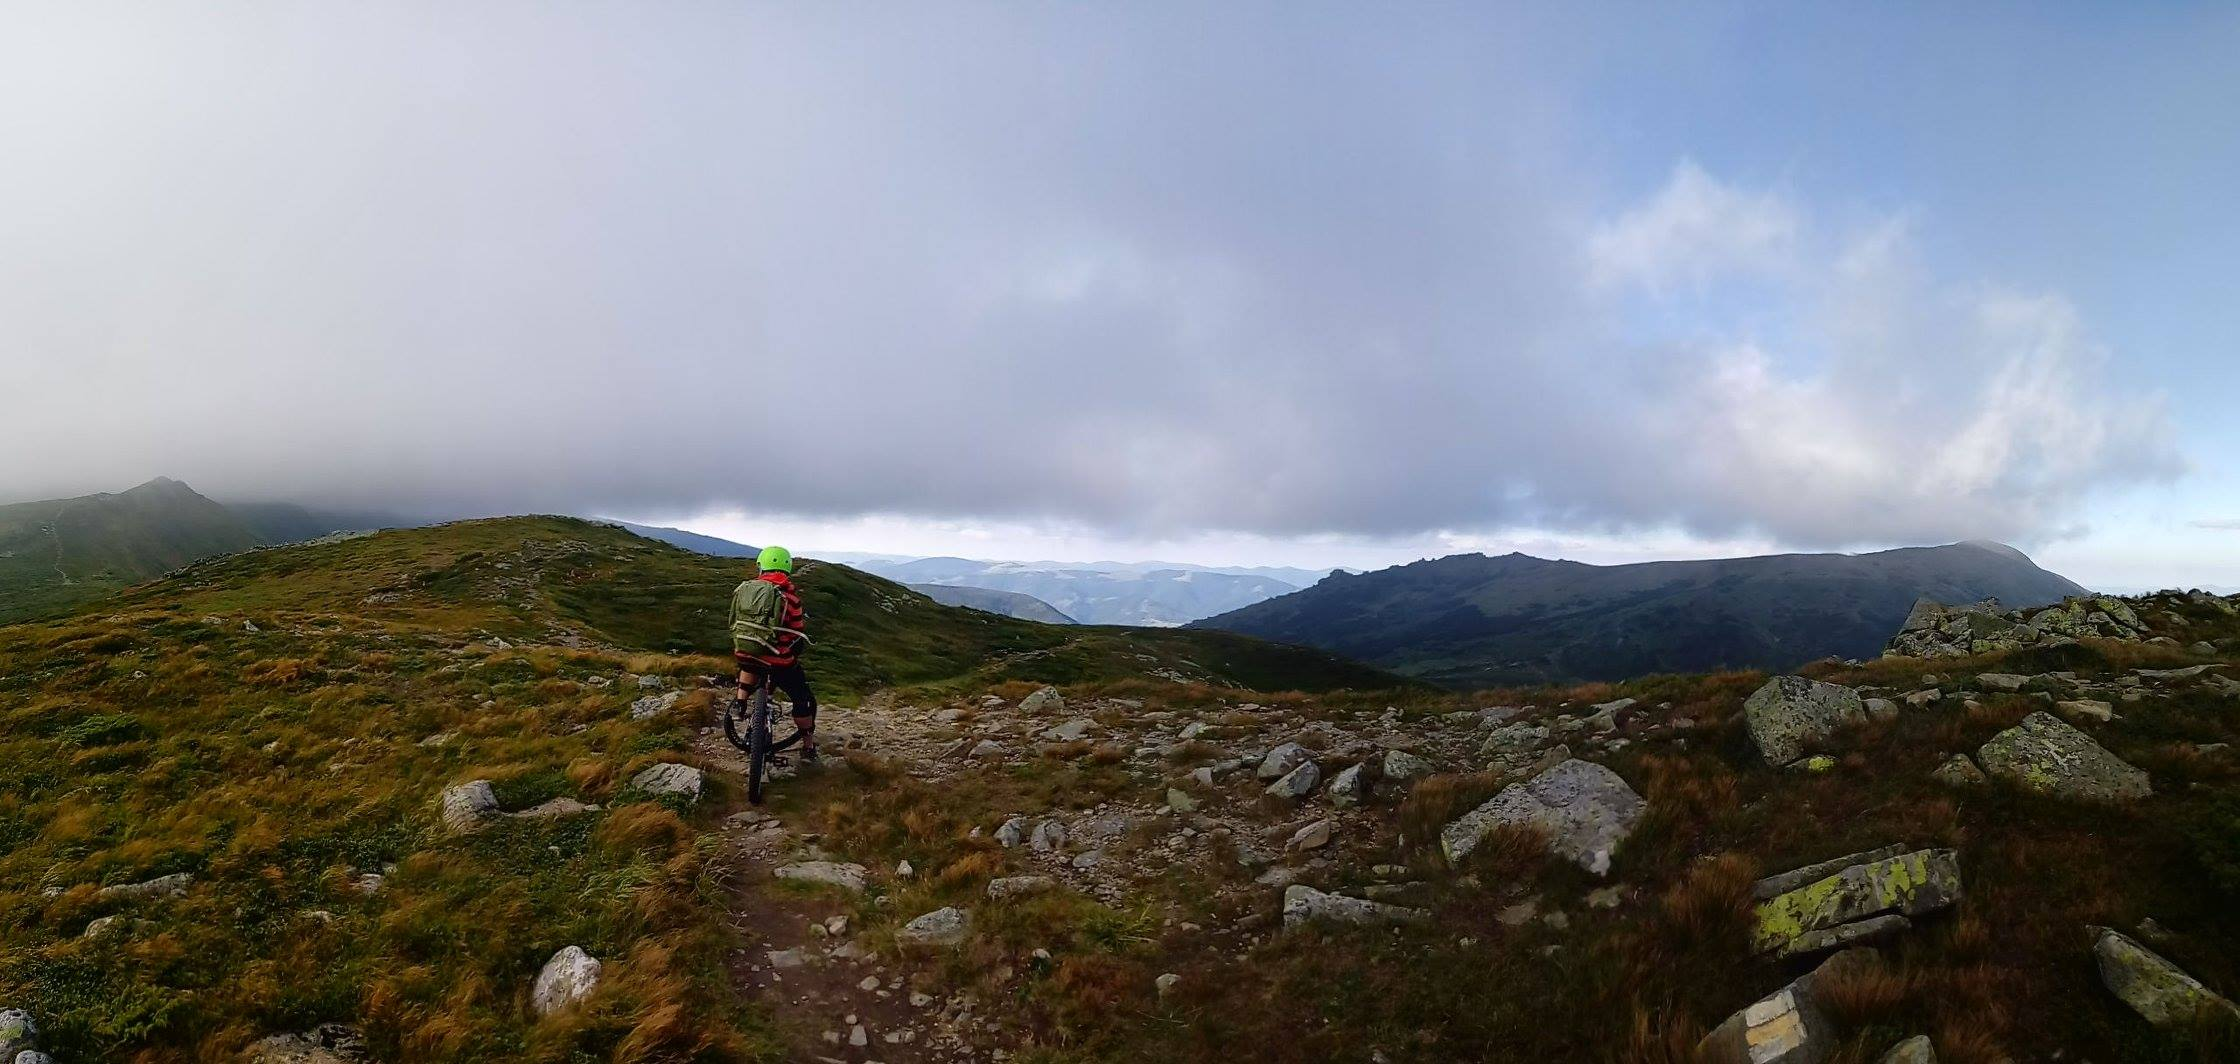
\includegraphics[width=0.9\textwidth]{foto3}
\end{center}

\section{availability}
{I'm available since the 1st of October, but I may start working in the end of November as well. I'm going to move to Cracow now in order to live closer to the places and people I love.}

\section{legal}
{I hereby authorise you to process my personal data included in my job application for the needs of the current and future recruitment processes (in accordance with the Personnel Protection Act of 29.08.1997 no 133 position 883).}
\end{document}
